
In the following, we will summarise the results obtained for the IRTF
data set. We deal with the different physical paramenters in separate
Sections. We start by reporting the cross validation Root Mean Square
Errors (RMSE) for the ?-fold cross-validation strategy, and
subsequently discuss the accuracy of the predictions with respect to
literature values where available.

\subsection{Effective temperature models}

Table \ref{tab:model_TSD} summarises the RMSE for the complete set of
models: the minimum $\chi^2$ estimate based on the full spectrum
($\chi^2$), the projection pursuit regression based on the ICA
components (PPR-ICA), the {\bf ???? Joaquín, fill here the details,
and also in meth.tex} model trained of the spectral features
by \cite{cesetti} (C-???), and the 8 models trained on the spectral
features proposed by the GA (GA-GAM, GA-MARS, GA-RF, GA-BOOSTING,
GA-GBM, GA-SVM, GA-SVM, GA-NNET, GA-KPLS). For each model, we report
the RMSE obtained for several noise levels of the training and test
sets. We use the following notation: RMSEaa represents the RMSE
obtained for a model trained and tested on BT Settl spectra of
SNR=aa. SNR=$\infty$ corresponds to noiseless spectra. The prefix CV-
corresponds to cross-validation RMSE, and LI- to RMSE derived by
comparison with the literature values gathered by \cite{cesetti}.

\begin{table}
\begin{center}
\begin{tabular}{rrrrrrrrrrrr}
  \hline
  
  SNR & $\chi^2$ & PPR-ICA & C-??? & GA-RF & GA-GBM & GA-SVM & GA-NNET & GA-KNN & GA-MARS & GA-KPLS & GA-RULE \\

\hline

CV-RMSE$\infty$ &        &        &  & 232.10 & 233.22 & 299.05 & 326.35 & 219.14 & 226.14 & 387.06 & 332.92\\
CV-RMSE10 & 232.55 & 241.93 &  & 308.46 & 287.21 & 221.46 & 283.44 & 238.18 & 253.14 & 275.48 & 260.76\\
CV-RMSE50 & 235.25 & 241.83 &  & 247.65 & 247.93 & 281.21 & 264.16 & 232.36 & 254.00 & 299.88 & 270.09\\
LI-RMSE$\infty$ &  &  &  &  &  &  &  &  &  &  & \\
LI-RMSE10 &  &  &  &  &  &  &  &  &  &  & \\
LI-RMSE50 &  &  &  &  &  &  &  &  &  &  & \\

\hline
\end{tabular}
\caption {RMSE for the various regression models that predict $T_{eff}$ (K).} 
\label{tab:model_TSD} 
\end{center}
\end{table}

Table \ref{tab:model_TSD} shows that the performance of classifiers
based on the full spectrum (or in a compressed version in the form of
ICA components) and on features derived from limited spectral bands is
equivalent. The difference between the performances of best classifier
(GA-KNN; best on average over SNR), the minimum $\chi^2$ classifier,
and the PPR-ICA classifiers are not statistically significant. We
interpret these small differences as an indication that there is as
much information spread over the entire spectrum shape as can be
distilled from a few spectral bands. In any case, it is evident that
the RMSE is significantly above the grid spacing in temperature ({\bf
I think this is 100K but it depends on the answer to my questions
whether the interpolated grid was used or not.})

The comparison with the effective temperatures compiled
by \cite{cesetti} does not show significant differences either. In
general, all classifiers tend to predict lower effective temperatures
than those in the literature.{\bf Joaquín: ¿podemos calcular el sesgo
medio?} Most models show remarkably similar distributions of the
predictions when trained with different SNR levels. In the cases of
GA-MARS, GA-KNN, and GA-SVR this is the case even in the unrealistic
scenario of SNR=$\infty$.

In general, models tends to produce better behaved solutions (with
smaller biases and less scatter) for SNR=50. We interpret this value
as representative of the SNR of the majority of spectra in the IRTF
collection. We have found in previous studies that, at least for input
spaces constructed from ICA compressions of the spectra, it is not
necessary to adapt the training set SNR to match exactly that of the
prediction set. On the contrary, we find that two regimes are
sufficient to obtain optimal results. The two regimes are separated at
SNR=10. The model trained with SNR=50 spectra gives close to optimal
results for spectra with SNRs above 10, while below that limit the
same situation applies holds for the model trained with SNR=10
spectra. {\bf I should move this explanation to the beginning of the
section or to the methodology section. Joaquín: can you check that
what I am saying about Ana's results is correct?}




%\begin{table}
%\begin{center}
%\begin{tabular}{rrrrrrr}
%  \hline
%  SNR & Features & SVM & RF & GAM  & MARS  \\
%  \hline
%  \multirow{2}{*}{50}  &  Cesetti et al. & 81.6 &  83.3 & 163.5 & 91.9 \\
%      &  GA             & 91.4 & 82.2 & 161.1  & 91.9  \\
%  \multirow{2}{*}{10}  &  Cesetti et al. & 135.8 & 138.5 & 268.8 & 166.8  \\
%      &  GA             & 123.2 & 122.6 & 212.6 & 130.9  \\
%   \hline
%\end{tabular}
%\caption { RSME for different models predicting $T_{eff}$ [K].} 
%\label{tab:model_TSD} 
%\end{center}
%\end{table}

%After calculating the bartlett test for both cases of SNR it was 
%seen that variances are homogeneous since p > 0.05, and 
%the Flinger-Killen shows that homokedascity is verified, 
%then F-ANOVA test makes clear that there is no significative 
%difference between models. Then, it is possible to conclude
%that quality of features from both sources are equivalent
%regarding modeling capability, even when GA only has proposed five
%features and Cesetti et al. requires seven features.

%As an alternative to build modles based on bandpasses, 
%a similiar methodology to the one depicted in (\cite{2013A&A...550A.120S})
%was implemented.

%For the projection an Independend Component Analysis (ICA) with ten dimensions
%was used and for Temperature regression an optimized SVM 
%with parameters of C=10 and $\epsilon$=0.001.

%Considering the Gravity case, the most suitable ICA had twentysix dimensions and the 
%best SVM parameters were C=1000 and $\epsilon = 0.001 $. This was the same case
%for Metallicity.

%In terms of interpretation, this methodology looks to predict the physical paramenters
%by considering the whole star spectrum instead of information provided 
%by specific bands. Thus it can be interesting to analyze suitability 
%for prediction against the other approach.

%In the same sense it was decided to consider direct selection, which is
%also a technique based on the whole espectrum but, instead of regressing
%specific parameters, the closest labeled spectrum to the one 
%under analysis is identified by a $\chi^2$ distance.
%This becomes possible as interpolation between labeled spectra can be
%easily performed.

We then compare the predicted effective temperatures with the spectral
types listed in the IRTF spectral library. We attempted a direct
comparison with the literature values gathered in \cite{cesetti} but
it only returns {\bf ???? Joaquín, rellena este valor por favor}
estimates of effective temperature for M stars. We converted the
spectral types into effective temperatures using the calibration
of \cite{2009ApJ...702..154S}.

{\bf TODO: Luis, cambiar spectral libraries por stellar atmosphere
models o synthetic spectral libraries}.

Forecast quality of models was tested by the error against the
temperature estimated based on the Spectral Subtype for each of the
IRTF available spectra (see \ref{ssub:TLSB}).  Both Root Mean Squared
Error (RMSE) and Mean Absolute Error (MAE) where calculated and it is
presented in the table~\ref{tab:model_Tvar}.

From this comparison several things arise:
\begin{itemize}
 \item {The behavior of $\chi^2$ distance is quite stable against SNR 
	in the original dataset (BT\_Settl) with a slightly better global 
	performace in fovour of SNR=50.}
 \item {Models trained with different SNR=$\infty$ have similar performance but heavy 
	differences appear when SNR features are considered.}
 \item {When synchronous behavior is observed FT00, FT11, FT55, the better SNR is 10.}
 \item {Best set of features to be used for forecast are those from SNR=$\infty$ (FT0b).}
 \item {As a conclusion the better performance was produced by FT01, followed by the FT51.}
\end{itemize}

In Figure~\ref{fig:comp01} the relationship between Temperature
estimated from the GA model proposed features with SNR=50 and features
from SNR=$\infty$ and the Temperature estimation from spectral subtype
in comparison with the $chi^2$ with SNR=50 can be seen.

\begin {figure}
 \centering
 \begin{subfigure}{.85\textwidth}
  \centering
  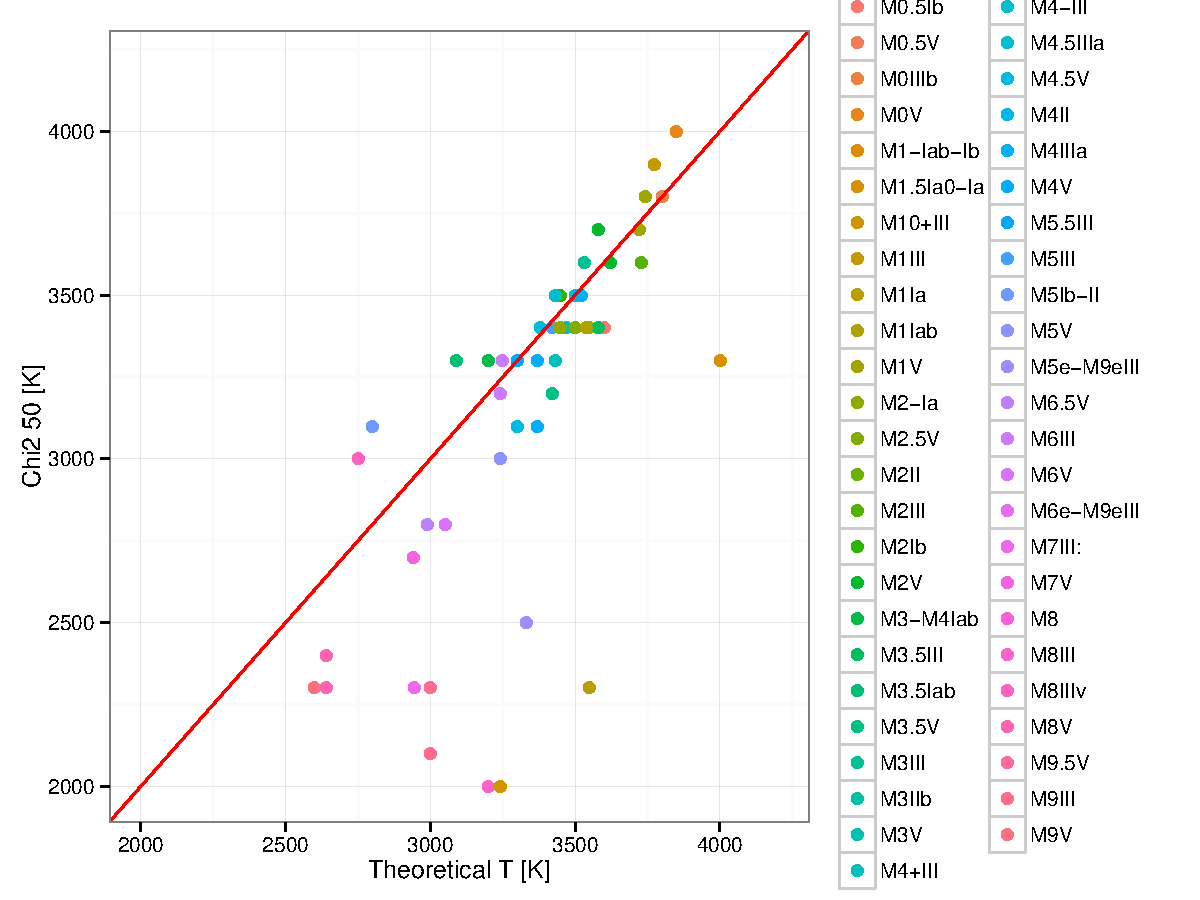
\includegraphics[width=13cm]{figs/T_chi50_Tst.pdf}
  \caption{Comparison between Temperature estimations from Spectral Subtype 
 in x axis and the closest BT\_Settl spectra by $\chi^2$ at SNR=$50$ on y-axis}
 \label{fig:chi2_50_spt}
 \end{subfigure}
  \begin{subfigure}{.85\textwidth}
  \centering
  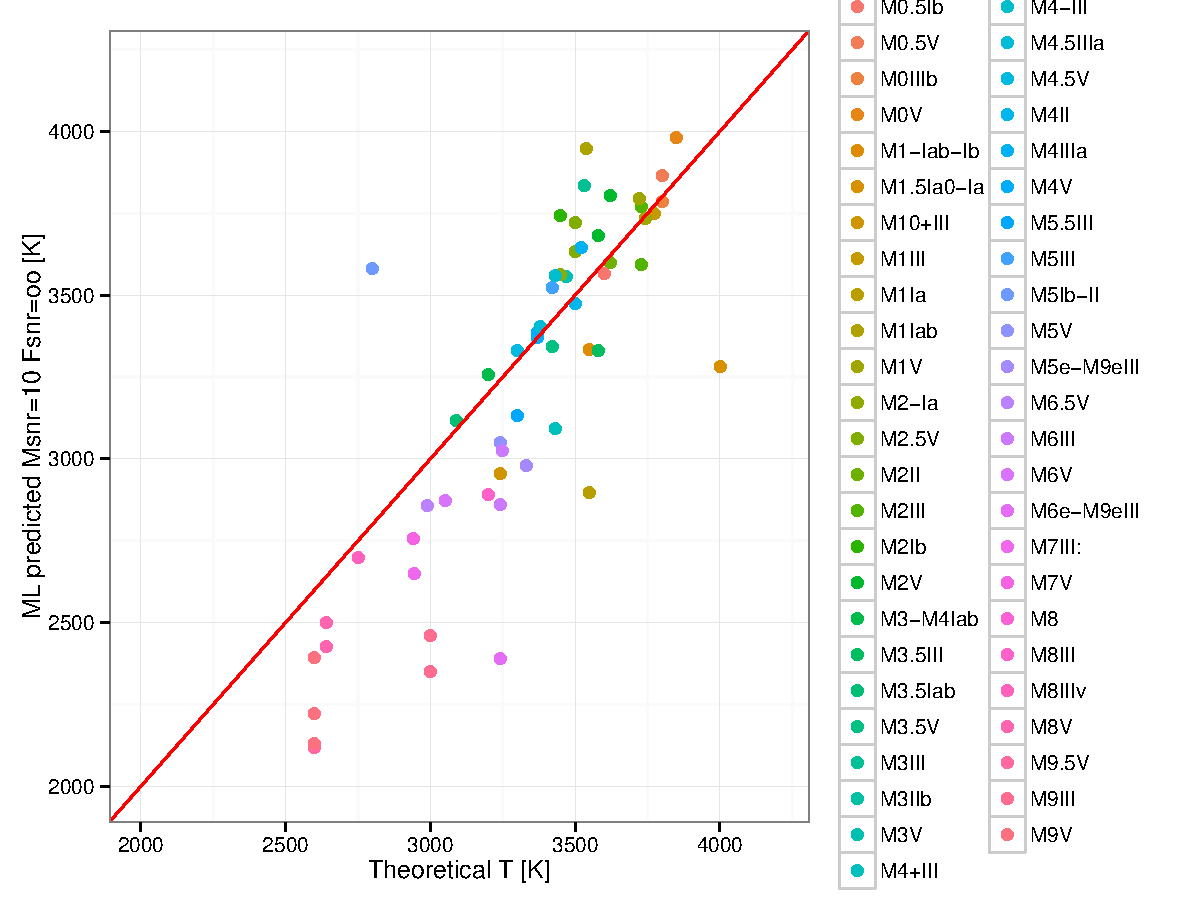
\includegraphics[width=13cm]{figs/T_svm_10_TsP.pdf}
  \caption{Comparison between Temperature estimations from Spectral Subtype 
 in x axis and the Support Vector Machines for Ga based features trained with BT\_Settl 
 at SNR=$\infty$ and features for forecasting at SNR=10 on y-axis}
 \label{fig:ga_too50ga_spt}
 \end{subfigure}
 \label {fig:comp01}
 \caption{Performance comparison between the $chi^2$ based selection 
          and the band oriented features}
\end {figure}
%
% No le añado más discusión porque habría que interpretar algunas estrellas.
%

% En kile ^D Comenta y ^MayD descomenta
%
% Similarly Figure~\ref{fig:t10ga_tsb} shows the relationship against GA features 
% and Random Forest model trained by BT-Settl at SNR=10.
% 
% \begin {figure}
%  \begin{center}
%  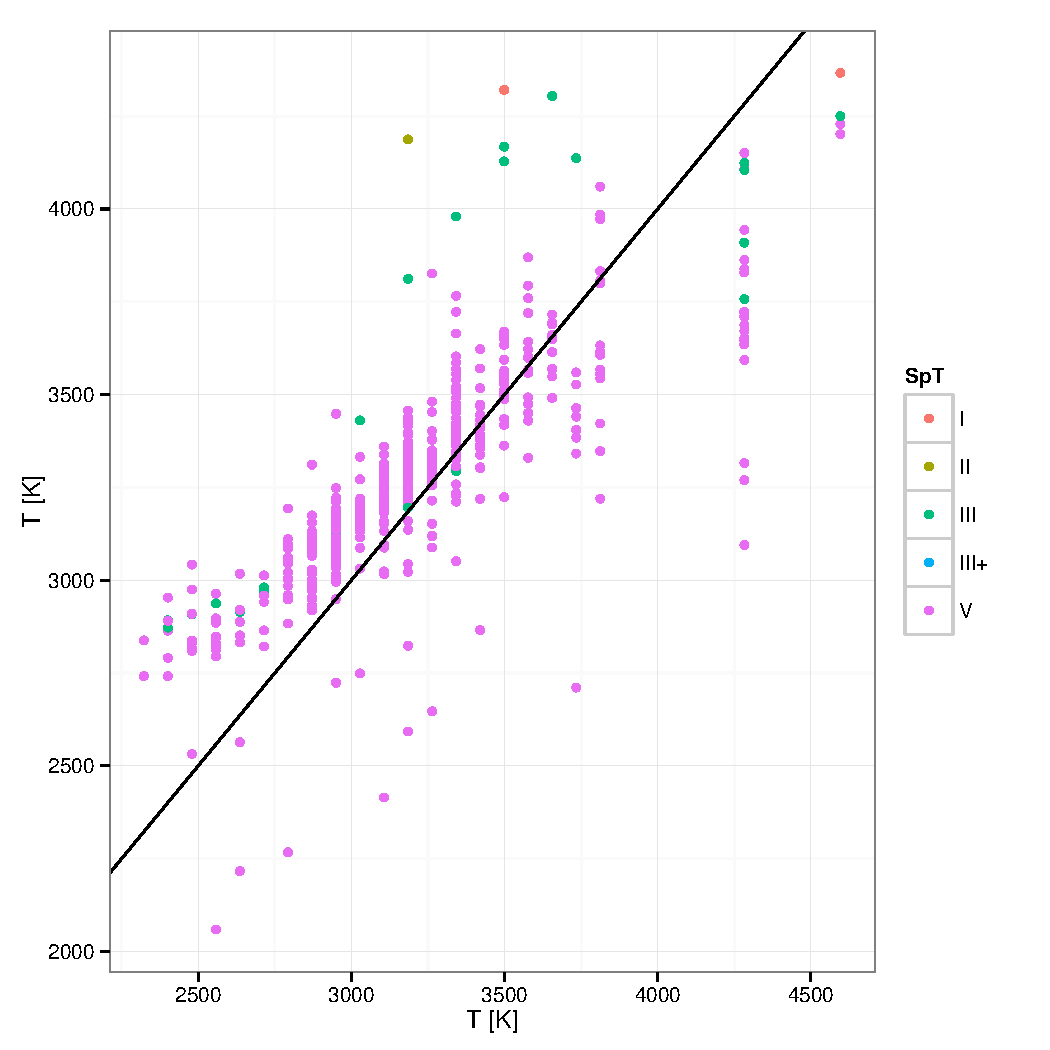
\includegraphics[width=6cm]{figs/T10GA_TSB.pdf}
%  \caption{Comparison between Temperature estimations from Spectral Subtype 
%  in x axis and the Random Forest for Ga based features trained with BT-Settl 
%  at SNR=10 on y-axis}
%  \label{fig:t10ga_tsb}
%  \end{center}
% \end {figure}


The comparison against processing the whole spectrum by ICA projection 
has been performed and the results for SNR=\{10,50\} can be seen 
in Figure~\ref{fig:T_ICA_10_SpT} and Figure~\ref{fig:T_ICA_50_SpT}.

\begin {figure}
 \centering
 \begin{subfigure}{.85\textwidth}
  \centering
  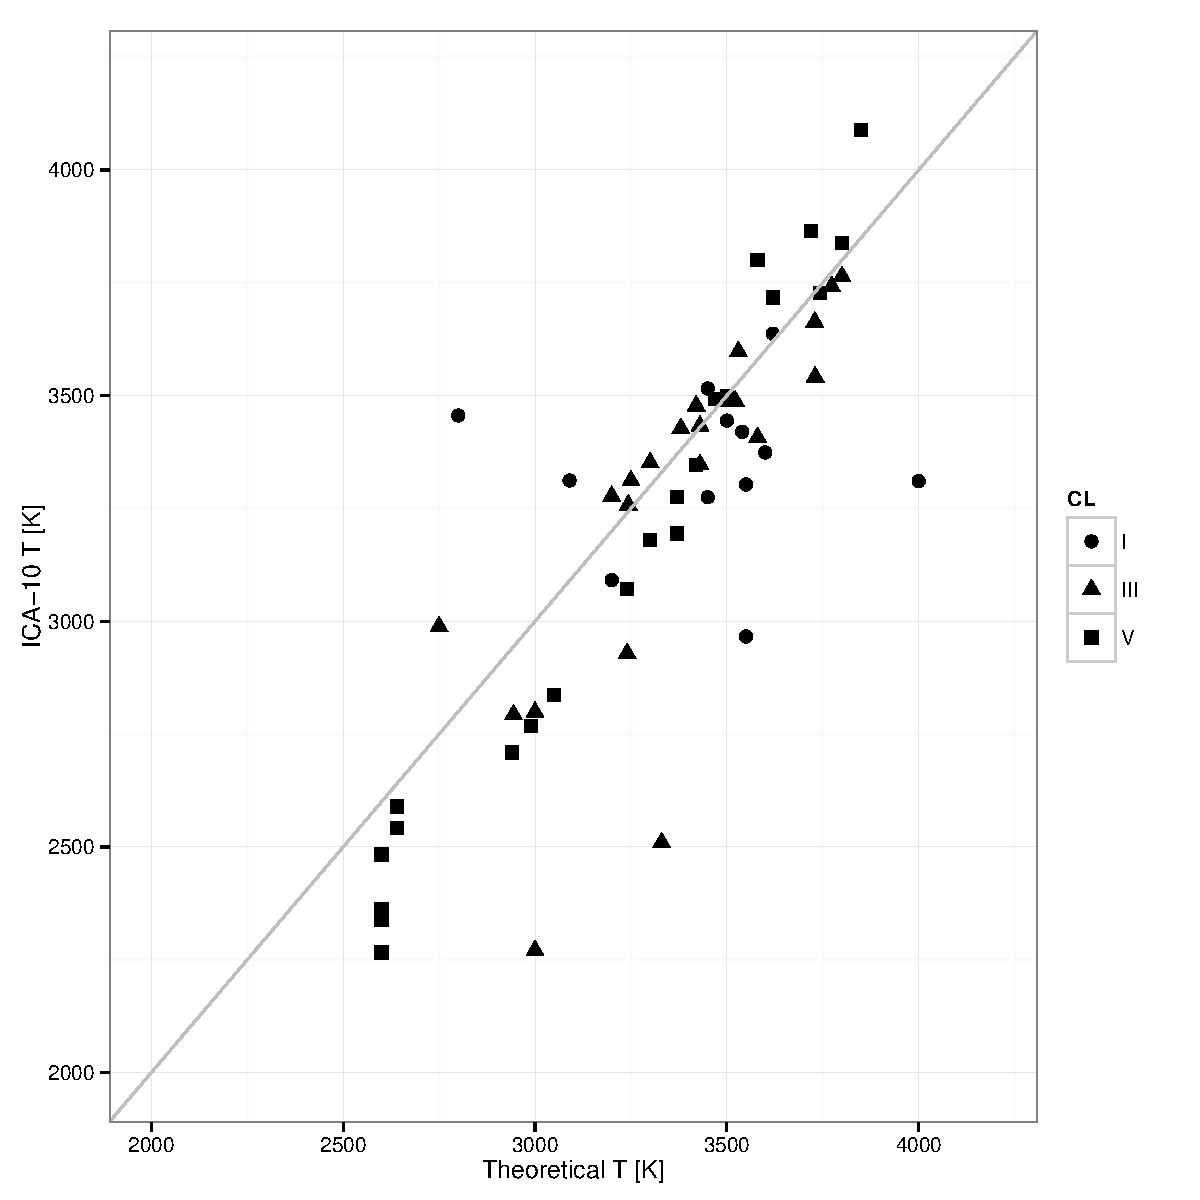
\includegraphics[width=12cm]{figs/T_ICA_10_SpT.pdf}
  \caption{Comparison between Temperature estimations from Spectral Subtype 
 in x axis and the prediction based on SVM models over the ICA projection 
 with 10 components at SNR=$10$ on y-axis}
 \label{fig:T_ICA_10_SpT}
 \end{subfigure}
  \begin{subfigure}{.85\textwidth}
   \centering
  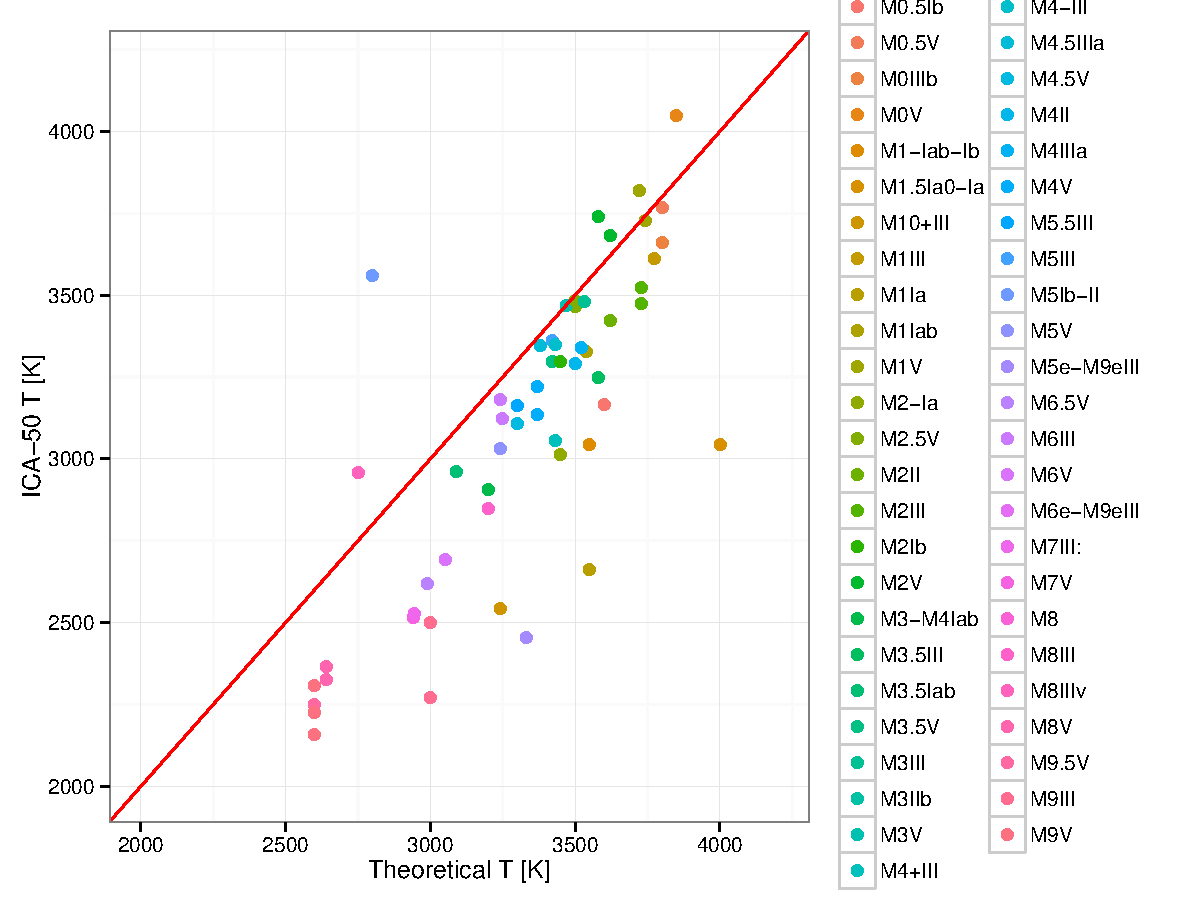
\includegraphics[width=12cm]{figs/T_ICA_50_SpT.pdf}
  \caption{Comparison between Temperature estimations from Spectral Subtype 
 in x axis and the prediction based on SVM models over the ICA projection 
 with 10 components at SNR=$50$ on y-axis}
 \label{fig:T_ICA_10_SpT}  
  \end{subfigure}
 \label{fig:t_ica_1050_SpT}
\end {figure}

% No le añado más discusión de momento, hasta ver si tiene sentido poer toda esta
% fila de gráficas o es mejor producir algo más condensado.
%

\subsection{Surface gravity models}

The same approach can become useful to produce $log(G)$ estimations. 
Here comparisons can only be possible between GA based features, the 
global spectra based approach with $\chi^2$ distance
to be minimized and those stars with gravity was 
estimated in  \cite{2013A&A...549A.129C}.

The only difference with the methodology presented above is because
Temperature has been considered a fixed feature in the estimation of 
Gravity.

In Tables~\ref{tab:models_G_rmse} and~\ref{tab:models_G_mae} 
we can see the analysis of performance between
the $\chi^2$ identificacion and the one based on features from the spectrum
depending on several classes of features.

\begin{table}[ht]
\centering
\begin{tabular}{rrrrrrrr}
  \hline
 & rf & gbm & boosting & svm & gam & nnet & mars \\ 
  \hline
G\_chi2\_10 & 1.68 & 1.68 & 1.68 & 1.68 & 1.68 & 1.68 & 1.68 \\ 
  G\_chi2\_50 & 1.79 & 1.79 & 1.79 & 1.79 & 1.79 & 1.79 & 1.79 \\ 
  FG00 & 2.01 & 1.62 & 2.32 & 1.78 & 0.98 & 3.39 & 2.13 \\ 
  FG01 & 2.52 & 2.56 & 2.62 & 1.87 & 2.52 & 2.32 & 2.45 \\ 
  FG05 & 2.49 & 2.42 & 2.40 & 1.78 & 2.29 & 2.89 & 2.16 \\ 
  FG10 & 2.34 & 2.59 & 2.75 & 1.78 & 32.52 & 3.39 & 3.04 \\ 
  FG11 & 2.49 & 2.48 & 2.69 & 1.90 & 2.67 & 2.50 & 2.57 \\ 
  FG15 & 2.75 & 2.72 & 2.51 & 1.78 & 2.95 & 3.94 & 2.52 \\ 
  FG50 & 2.61 & 2.11 & 2.58 & 1.78 & 17.95 & 3.39 & 6.07 \\ 
  FG51 & 2.78 & 2.82 & 2.77 & 1.92 & 2.73 & 2.43 & 2.65 \\ 
  FG55 & 2.58 & 2.57 & 2.71 & 1.78 & 2.80 & 2.34 & 2.63 \\ 
   \hline
\end{tabular}
\caption { RMSE for different models predicting $Log(G)$ [dex].} 
\label{tab:models_G_rmse} 
\end{table}

\begin{table}[ht]
\centering
\begin{tabular}{rrrrrrrr}
  \hline
 & rf & gbm & boosting & svm & gam & nnet & mars \\ 
  \hline
G\_chi2\_10 & 1.46 & 1.46 & 1.46 & 1.46 & 1.46 & 1.46 & 1.46 \\ 
  G\_chi2\_50 & 1.46 & 1.46 & 1.46 & 1.46 & 1.46 & 1.46 & 1.46 \\ 
  FG00 & 1.78 & 1.50 & 2.05 & 1.54 & 0.82 & 3.06 & 1.84 \\ 
  FG01 & 2.14 & 2.19 & 2.27 & 1.75 & 2.18 & 1.80 & 2.07 \\ 
  FG05 & 2.13 & 2.07 & 2.07 & 1.35 & 1.59 & 2.70 & 1.54 \\ 
  FG10 & 2.09 & 2.31 & 2.43 & 1.54 & 27.48 & 3.06 & 2.73 \\ 
  FG11 & 2.12 & 2.16 & 2.34 & 1.77 & 2.30 & 2.03 & 2.17 \\ 
  FG15 & 2.35 & 2.29 & 2.17 & 1.35 & 2.52 & 3.64 & 1.86 \\ 
  FG50 & 2.50 & 1.99 & 2.23 & 1.54 & 15.75 & 3.06 & 4.03 \\ 
  FG51 & 2.46 & 2.48 & 2.43 & 1.79 & 2.50 & 1.89 & 2.37 \\ 
  FG55 & 2.15 & 2.16 & 2.34 & 1.35 & 2.48 & 2.05 & 2.29 \\ 
   \hline
\end{tabular}
\caption { RMSE for different models predicting $Log(G)$ [dex].} 
\label{tab:models_G_mae} 
\end{table}



It is possible to present relationships between $log(g)$ and $log(T_{eff})$
as a matter of congruence analysis between predictions. In the Figure~\ref{fig:lt_lg_ga}
such relationship is presented for models based on artificial intelligence selected features.
In Figure~\ref{fig:lt_lg_chi2} the values for $log(T_{eff})$ and $log(G)$ are 
inferred from the closest BT\_Settl spectra.

\begin{figure}
 \begin{center}
 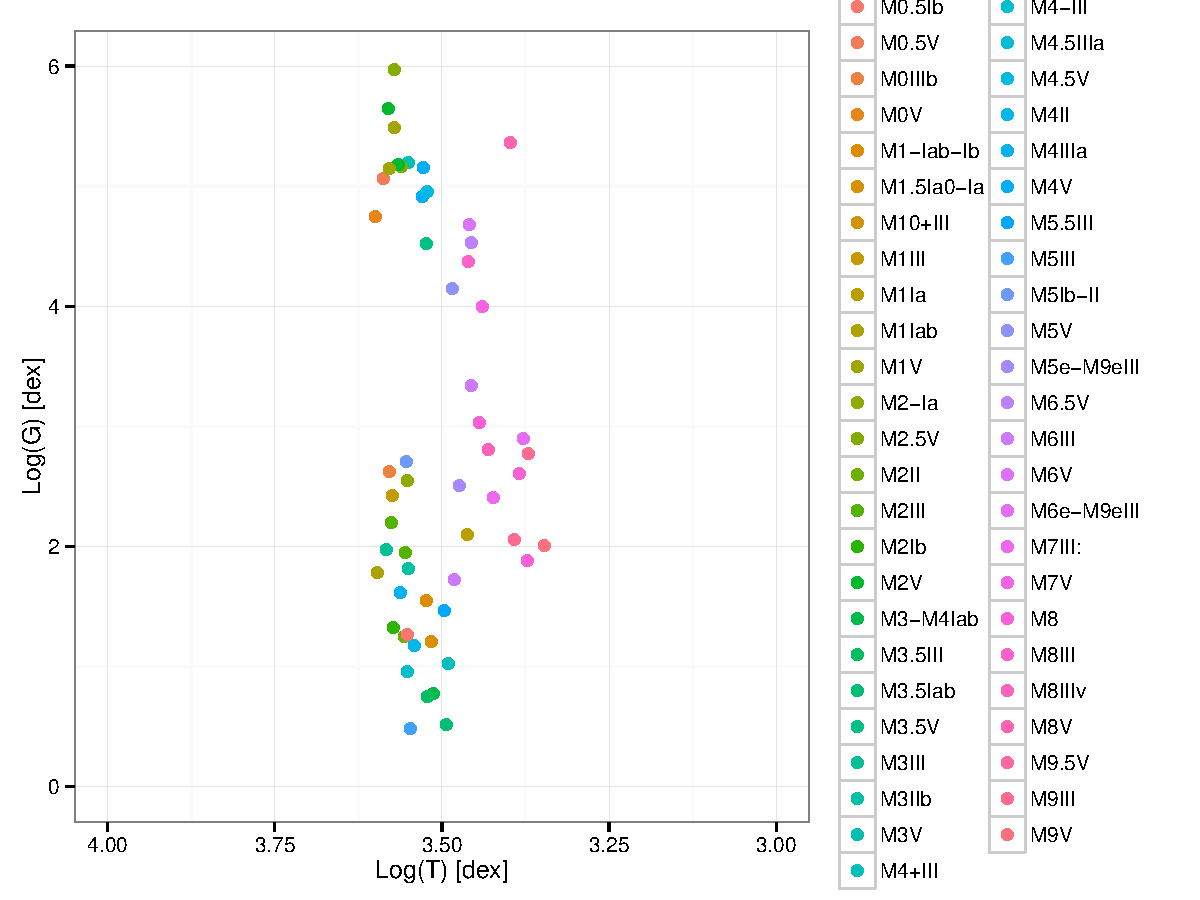
\includegraphics[width=12cm]{figs/LT_LG_ga.pdf}
 \caption{Relationship between $log(T_{eff}) $ in the x axis 
 and $log(g)$ in the y axis for models based on bandpass features }
 \label{fig:lt_lg_ga}
 \end{center}
\end{figure}

And, for sure, it is possible to do it for estimations based on 
parameters from nearest labeled BT-Settl spectra.
In this particular case, it is possible to see how 
considering the global spectrum is positive for stronger 
physical parameters like $T_{eff}$ but the approach
reduces drastically its likelihood when other softer 
parameters are involved.

\begin{figure}
 \begin{center}
 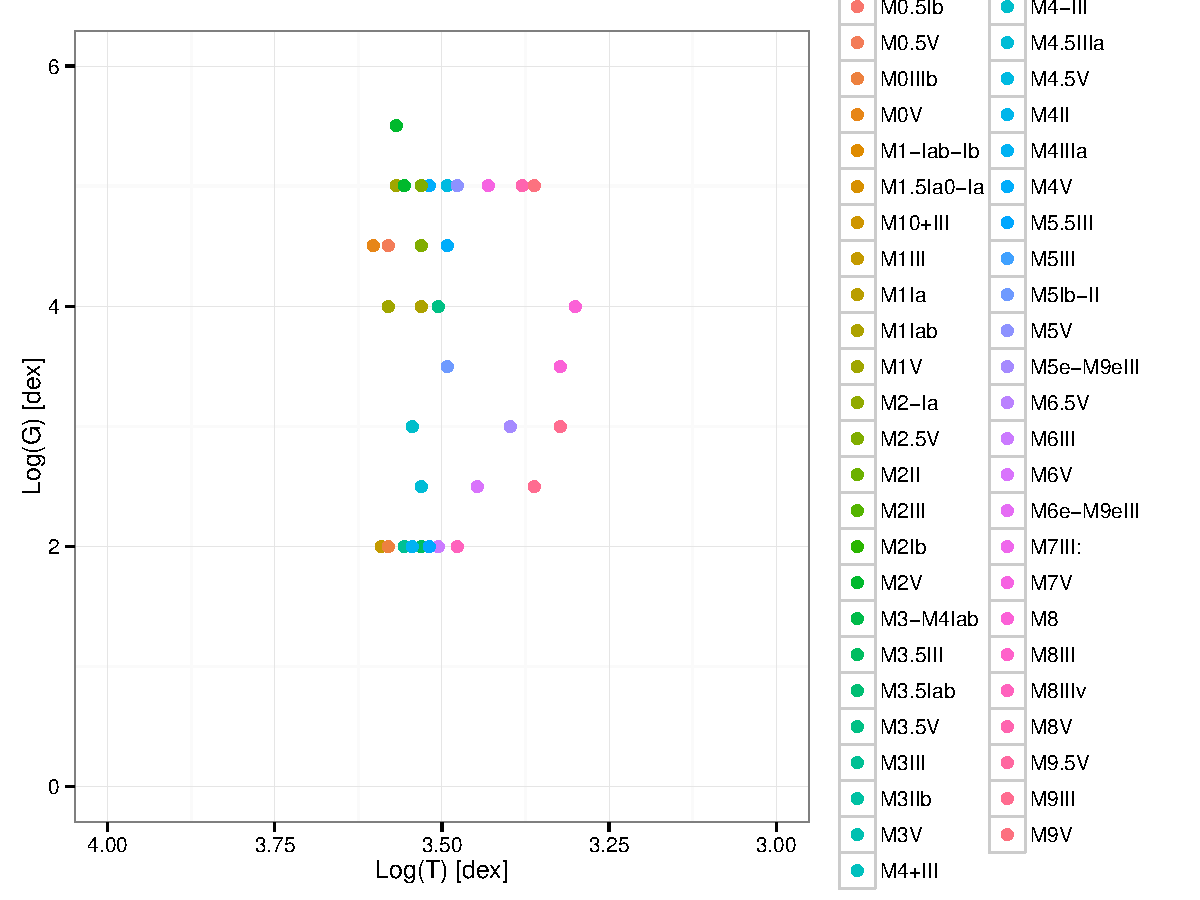
\includegraphics[width=12cm]{figs/LT_LG_chi2.pdf}
 \caption{Relationship between $log(T_{eff}) $ in the x axis 
 and $log(g)$ in the y axis for SNR=50 when 
 the nearest BT-Settl spectrum is used.}
 \label{fig:lt_lg_chi2}
 \end{center}
\end{figure}

% Se debe realizar una intepretación, pero dependerá 

In Figure~\ref{fig:chi2_50_spt} and Figure~\ref{fig:ga_too50ga_spt} 
relationships between $log(g)$ predicted by global espectrum estimation 
and GA feature based estimation can be observed.

\begin {figure}
 \centering
 \begin{subfigure}{.85\textwidth}
  \centering
  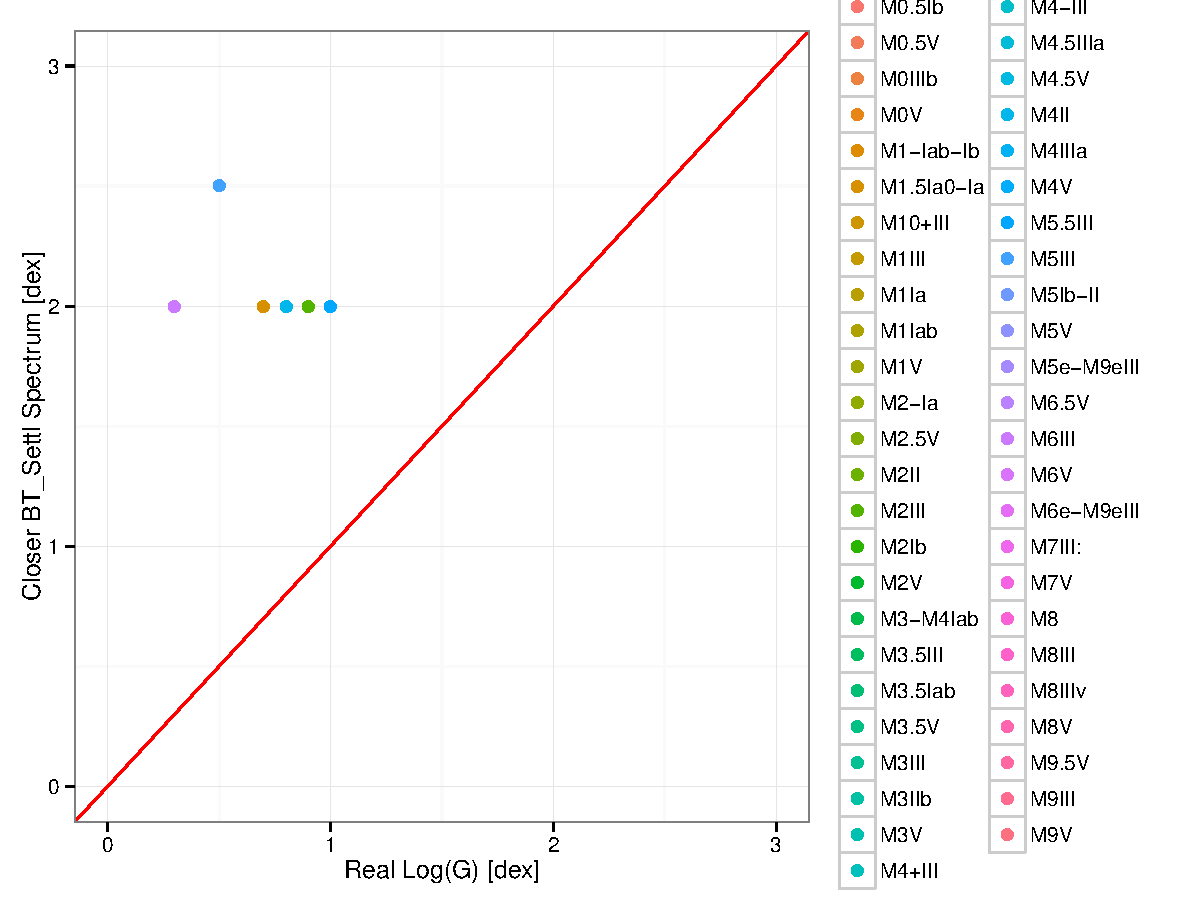
\includegraphics[width=12cm]{figs/G_chi2_50_cesetti.pdf}
  \caption{Comparison between Gravity estimations from Spectral Subtype 
 in x axis and the closest BT\_Settl spectra by $\chi^2$ at SNR=$50$ on y-axis}
 \label{fig:chi2_50_spt}
 \end{subfigure}
  \begin{subfigure}{.85\textwidth}
  \centering
  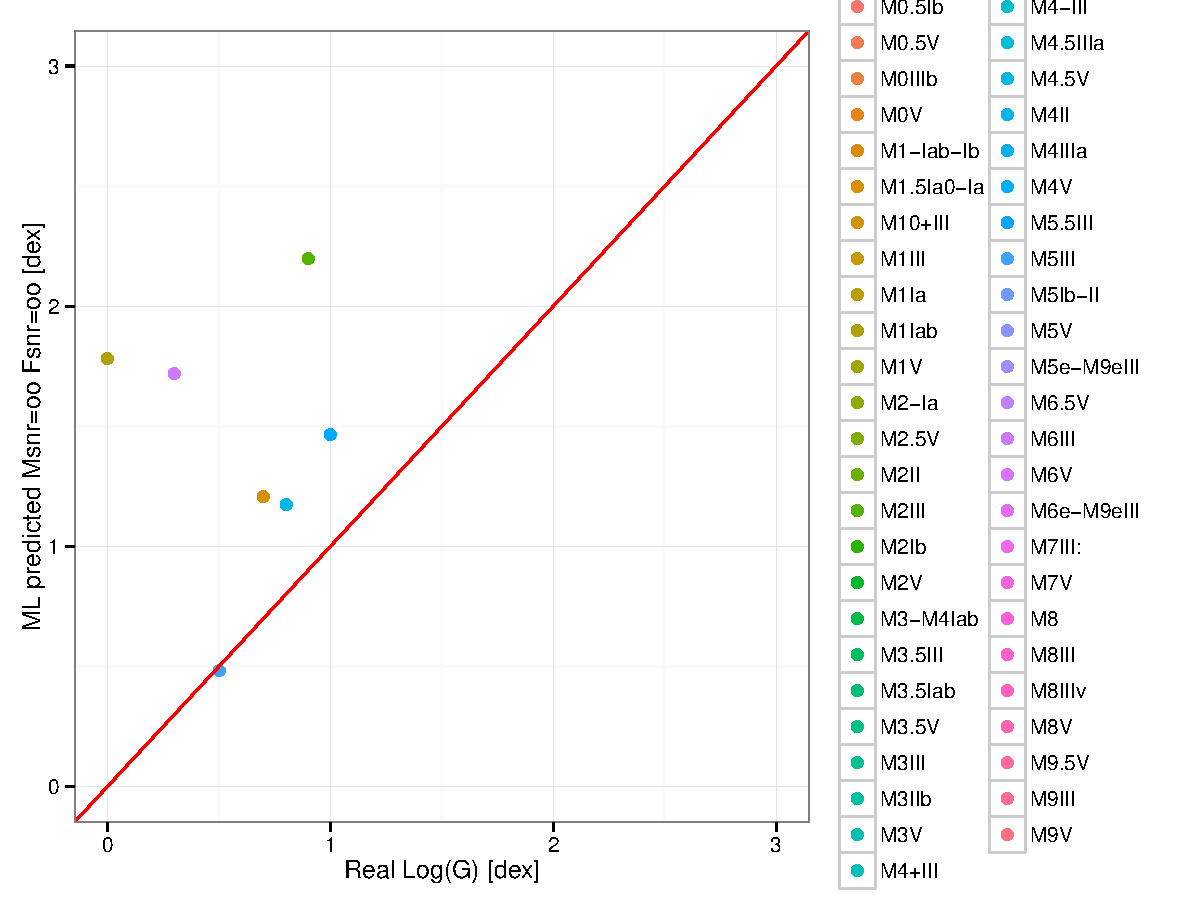
\includegraphics[width=12cm]{figs/G_gam_oo_cesetti.pdf}
  \caption{Comparison between Gravity estimations from Spectral Subtype 
 in x axis and the Support Vector Machines for Ga based features trained with BT\_Settl 
 at SNR=$\infty$ and features for forecasting at SNR=$\infty$ on y-axis}
 \label{fig:ga_too50ga_spt}
 \end{subfigure}
 \label {fig:comp02}
 \caption{Performance comparison between the $chi^2$ based selection 
          and the band oriented features to forecast Log(g)}
\end {figure}
%

% De nuevo las valoraciones deberían esperar a ver qué ponemos.

\subsection{Metallicity models} 

Finally, the same analysis is performed for the Metalicty parameter, 
again by considering Temperature as a fixed feature.
In Tables~\ref{tab:models_M_rmse} and~\ref{tab:models_M_mae} 
we can see the analysis of performance of different classes of
models and cosidering a variety in features.

\begin{table}[ht]
\centering
\begin{tabular}{rrrrrrrr}
  \hline
 & rf & gbm & boosting & svm & gam & nnet & mars \\ 
  \hline
M\_Chi2\_10 & 0.19 & 0.19 & 0.19 & 0.19 & 0.19 & 0.19 & 0.19 \\ 
 M\_Chi2\_50 & 0.35 & 0.35 & 0.35 & 0.35 & 0.35 & 0.35 & 0.35 \\ 
  FM00 & 0.30 & 0.43 & 0.28 & 1.04 & 2.19 & 0.51 & 1.03 \\ 
  FM01 & 0.51 & 0.46 & 0.44 & 0.74 & 0.76 & 0.99 & 50.64 \\ 
  FM05 & 2.05 & 2.85 & 1.31 & 1.89 & 3.46 & 7.56 & 6.46 \\ 
  FM10 & 1.09 & 1.02 & 0.94 & 1.04 & 10.75 & 1.65 & 13.49 \\ 
  FM11 & 0.47 & 0.39 & 0.49 & 0.74 & 0.31 & 0.45 & 43.43 \\ 
  FM15 & 1.91 & 2.73 & 1.08 & 1.89 & 4.65 & 13.27 & 16.95 \\ 
  FM50 & 0.82 & 0.87 & 0.43 & 1.04 & 6.10 & 2.25 & 11.87 \\ 
  FM51 & 1.02 & 1.10 & 0.56 & 0.74 & 2.29 & 3.44 & 119.29 \\ 
  FM55 & 1.70 & 3.14 & 1.15 & 1.89 & 7.64 & 7.00 & 12.04 \\ 
   \hline
   \end{tabular}
\caption { RMSE for different models predicting $Met$ [dex].} 
\label{tab:models_M_rmse} 
\end{table}
   


\begin{table}[ht]
\centering
\begin{tabular}{rrrrrrrr}
  \hline
 & rf & gbm & boosting & svm & gam & nnet & mars \\ 
  \hline
M\_Chi2\_10 & 0.17 & 0.17 & 0.17 & 0.17 & 0.17 & 0.17 & 0.17 \\ 
  M\_Chi2\_50 & 0.26 & 0.26 & 0.26 & 0.26 & 0.26 & 0.26 & 0.26 \\ 
  FM00 & 0.24 & 0.38 & 0.25 & 1.02 & 2.01 & 0.33 & 0.92 \\ 
  FM01 & 0.47 & 0.40 & 0.40 & 0.72 & 0.66 & 0.90 & 33.30 \\ 
  FM05 & 2.04 & 2.85 & 1.29 & 1.88 & 3.41 & 7.38 & 6.28 \\ 
  FM10 & 0.80 & 0.71 & 0.62 & 1.02 & 8.88 & 0.99 & 10.82 \\ 
  FM11 & 0.43 & 0.37 & 0.46 & 0.72 & 0.24 & 0.37 & 25.59 \\ 
  FM15 & 1.90 & 2.68 & 1.05 & 1.88 & 3.68 & 11.77 & 13.21 \\ 
  FM50 & 0.78 & 0.79 & 0.40 & 1.02 & 5.13 & 1.83 & 9.90 \\ 
  FM51 & 1.01 & 1.08 & 0.54 & 0.72 & 2.22 & 3.36 & 77.52 \\ 
  FM55 & 1.67 & 3.10 & 1.13 & 1.88 & 7.11 & 6.33 & 11.22 \\
   \hline
   \end{tabular}
\caption { MAE for different models predicting $Met$ [dex].} 
\label{tab:models_M_mae} 
\end{table}
   

In Figure~\ref{fig:M_chi2_50_cesetti} and Figure~\ref{fig:M_GAM_1010_Cesetti} 
relationships between metalicity predicted by global espectrum estimation 
and GA feature based estimation against the real values
provided by \cite{2013A&A...549A.129C} can be observed.

\begin {figure}
 \centering
 \begin{subfigure}{.85\textwidth}
  \centering
  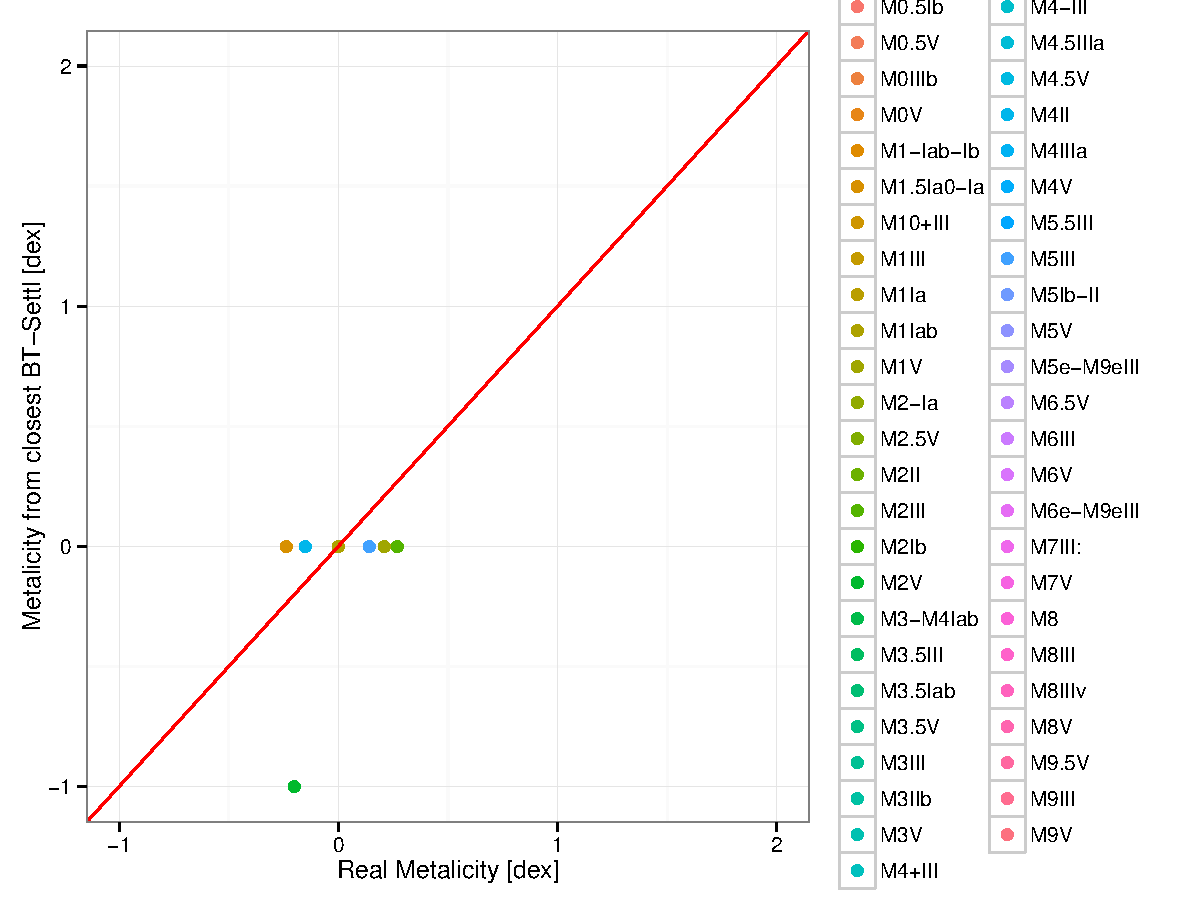
\includegraphics[width=12cm]{figs/M_Chi2_50_Cesetti.pdf}
  \caption{Comparison between Metalicity estimations from Spectral Subtype 
 in x axis and the closest BT\_Settl spectra by $\chi^2$ at SNR=$50$ on y-axis}
 \label{M_chi2_50_cesetti}
 \end{subfigure}
  \begin{subfigure}{.85\textwidth}
  \centering
  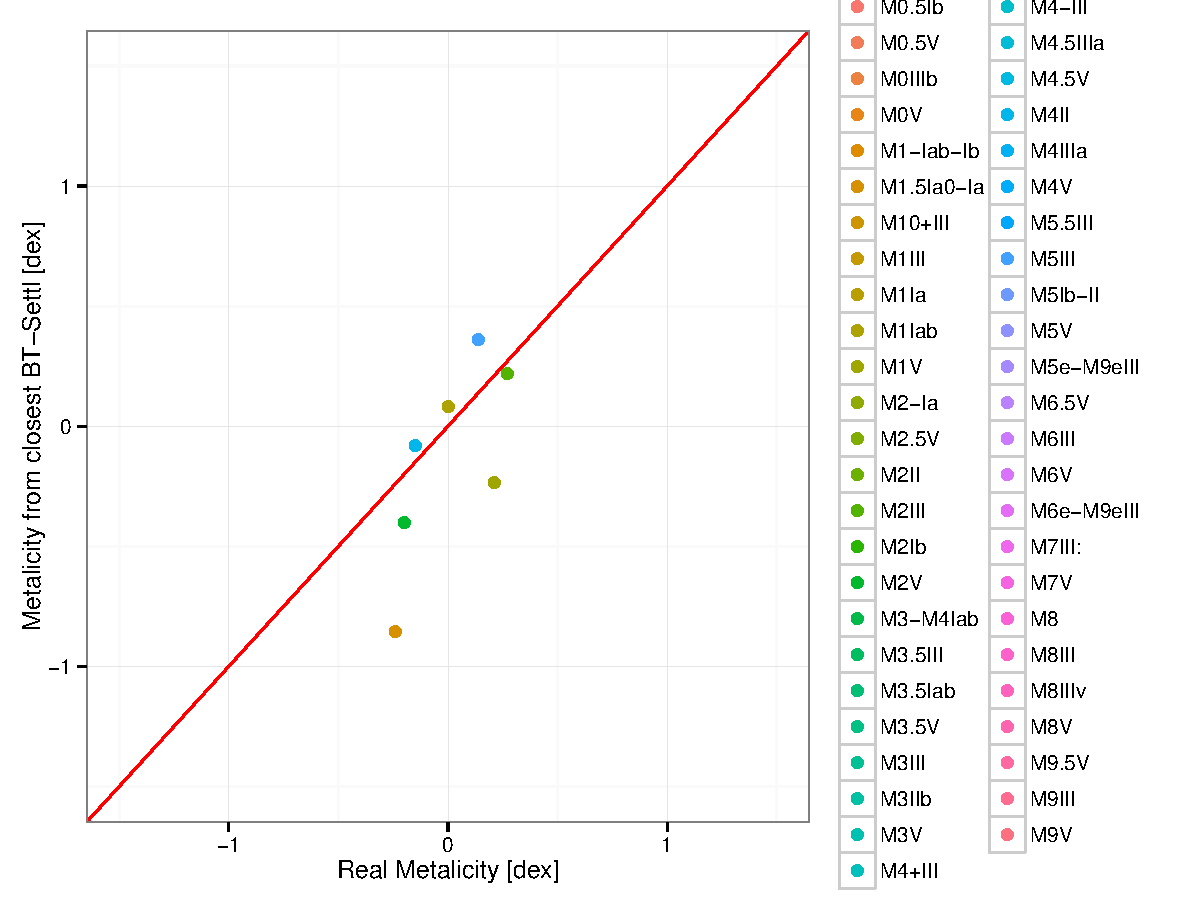
\includegraphics[width=12cm]{figs/M_GAM_1010_Cesetti.pdf}
  \caption{Comparison between Metalicity estimations from Spectral Subtype 
 in x axis and the Support Vector Machines for Ga based features trained with BT\_Settl 
 at SNR=$\infty$ and features for forecasting at SNR=$\infty$ on y-axis}
 \label{fig:M_GAM_1010_Cesetti}
 \end{subfigure}
 \label {fig:comp03}
 \caption{Performance comparison between the $chi^2$ based selection 
          and the band oriented features to forecast Log(g)}
\end {figure}
%
   
   

% De nuevo, el análisis y discusión, función de lo que queramos dejar

